\chapter{径流模型CaMaFlood}
%\addcontentsline{toc}{chapter}{陆地表面的水分循环}

汇流计算是通过耦合 Dai Yamazaki 等人于2011年提出的大尺度分布式汇流模型 CaMa-Flood (Catchment-based Macro-scale Floodplain) 实现的\citep{yamazaki2011physically}。
CaMa-Flood将全球河流网络分割为称为流域单元 (unit catchment) 的水文单元,在各单元集水区内利用河道 (river channel) 和漫滩 (floodplain) 的次网格 (subgrid) 
地形参数以及陆面模式生成的产流量 (total runoff),对总蓄水量 (total storage) 以及总流量 (total discharge) 进行预测,
并进一步实现对河道及漫滩流量 (river discharge and flood discharge),漫滩面积 (flood area) 以及平均漫滩水深 (flood depth) 
等日常所需的诊断量的高速计算。总蓄水量和总流量的时间演变通过求解局部惯性方程 \citep{bates2010} 得出。
CaMa-Flood同时考虑了上游单元的入流、下游单元的流出和每个流域单元的径流强迫输入,是目前高速求解河道水动力方程-圣维南方程最为高速有效的方法之一。
关于CaMa-Flood模型的详细描述可以从相关文献获取\citep{yamazaki2011physically,yamazaki2013improving,yamazaki2014regional,yamazaki2014development}。


CaMa-Flood 模型的主要优势之一在于除了能够精确描述河道径流以外,还能够模拟包括漫滩水位和漫滩面积变化等洪泛过程。
因此,对模拟结果的验证不仅仅局限于传统测量河流流量,还可以直接将模拟结果与卫星高度计对水面高程的观测以及微波成像仪对洪泛面积的估算进行比较;
能够有效加强全球河流模型各个输出的校准/验证\citep{yamazaki2012adjustment,yamazaki2012analysis}。
CaMa-Flood 模型的另一个优势在于它具有极高的模拟计算效率。通过引入次网格地形参数,复杂的漫滩淹没物理过程被合理地简化。
与此同时,通过实现局部惯性方程和自适应时间步长等物理方案\citep{bates2010},
河流流量和蓄水量的预测计算成本得到压缩,有利于进行集成/长期实验等计算要求高的实验或者与陆面模式之间的动态耦合。
以下对 CaMa-Flood 内部各个模块进行详细的介绍。目前耦合版本陆面过程模式分系统已经包含 CaMa-Flood v4.07版本。


\section{自适应时间步长的估算}
为避免固定时间步长计算所产生的数值振荡,提高数值方案稳定性,
CaMa-Flood 采用了\citet{bates2010}提出的基于局部惯性方程并满足 Courant-Friedrichs-Lewy (CFL) 
条件的自适应时间步长 ($DT_{adp}$) 的估算方法:
\begin{equation}
{DT}_{\max }=\boldsymbol{\alpha} \frac{\Delta x}{\sqrt{g h_{t}}}
\end{equation}
上式中$DT_{max}$是最大可接受的时间步长,$∆x$是该流域单元连接下游流域单元的河道长度 (river length) (m),
$\alpha$是稳定性系数设为0.9,$h_t$是该流域单元在时刻$t$的水流深度 (water depth) (m),$g$是重力加速度设为9.81 ($\rm m\,s^{-2}$)。
图~\ref{fig:自适应时间步长的估算} 展示了基于上述公式计算的某一时刻的$DT_{max}$ (minute)。
在计算过程中,如果用户指定的默认时间步长$DT$大于$DT_{max}$,则$DT$将被划分为满足$CFL$条件的更小的时间等分的时间步长$DT_{adp}$;
如果用户指定的默认时间步长$DT$小于$DT_{max}$,则实际计算步长按照用户指定的默认时间步长。
{
\begin{figure}[]
\centering
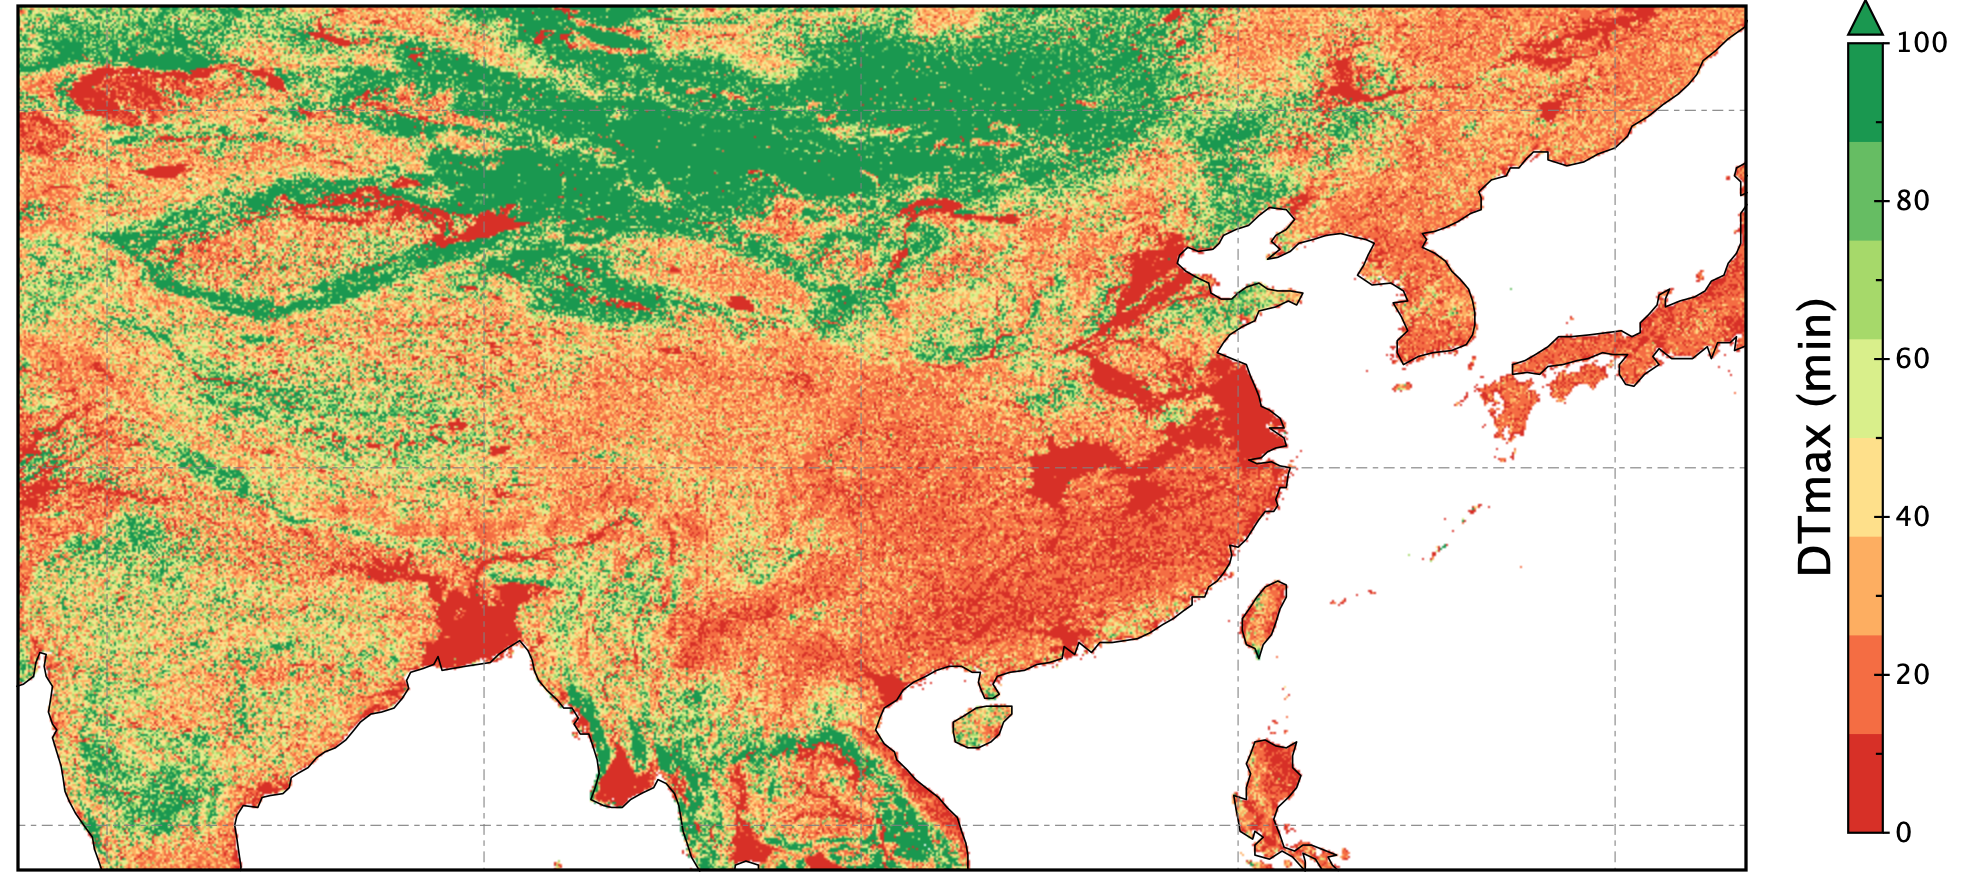
\includegraphics{Figures/陆地表面的水分循环/自适应时间步长的估算.png}
\caption{自适应时间步长的估算,摘自\citet{yamazaki2013improving}。}
\label{fig:自适应时间步长的估算}
\end{figure}
}


\section{诊断洪泛状态}\label{诊断洪泛状态}
在 CaMa-Flood 中指定网格的漫滩 (洪泛) 状态是通过计算该网格的蓄水总量得出的。如图~\ref{fig:CaMa-Flood流域单位示意图}
所示,河流河道蓄水量$S_r$,漫滩蓄水量$S_f$,河道水深度$D_r$, 漫滩淹没深度$D_f$,漫滩面积$A_f$等均通过求解基于总蓄水量的水量方程得出。
首先,模式中引发当前流域单元洪水蓄水量$S_{ini}$由如下公式进行确定:
\begin{equation}
S_{ ini }=B WL
\end{equation}
其中$B$是河道深度,$W$是河道宽度,及$L$是河道长度。如果总蓄水量$S$小于等于引发洪水蓄水量$S_{ini}$,
CaMa-Flood 假设不存在漫滩 (洪泛) 事件,上述参数则通过如下方程计算得出:
\begin{equation}
    \begin{array}{l}S_r=S \\ D_r=\frac{S_r}{WL} \\ S_f=0 \\ D_f=0 \\ A_f=0 \\ S_f=0\end{array}
\end{equation}
当总蓄水量$S$大于引发洪水蓄水量$S_{ini}$时,触发漫滩 (洪泛) 事件,则上述参数通过联立如下方程计算得出:
\begin{equation}
\begin{array}{l}S_r=S-S_f \\ D_r=\frac{S_r}{W L} \\ S_f=\int_{0}^{A_f}(D_f-D(A)) d_A \\ D_f=D_r-B \\ A_f=D^{-1}(D_f)\end{array}
\end{equation}
上式中的$D_f = D_r - B$表示河道与漫滩的水面高度相同。该方程是基于河道与漫滩之间的水量瞬间完成交换的假设。
函数$D^{-1}(D_f)$是漫滩高程剖面$D(A_f)$的反函数,它将泛滥地区$A_f$描述为漫滩水深$D_f$的函数 (见图~\ref{fig:CaMa-Flood流域单位示意图})。


{
\begin{figure}[]
\centering
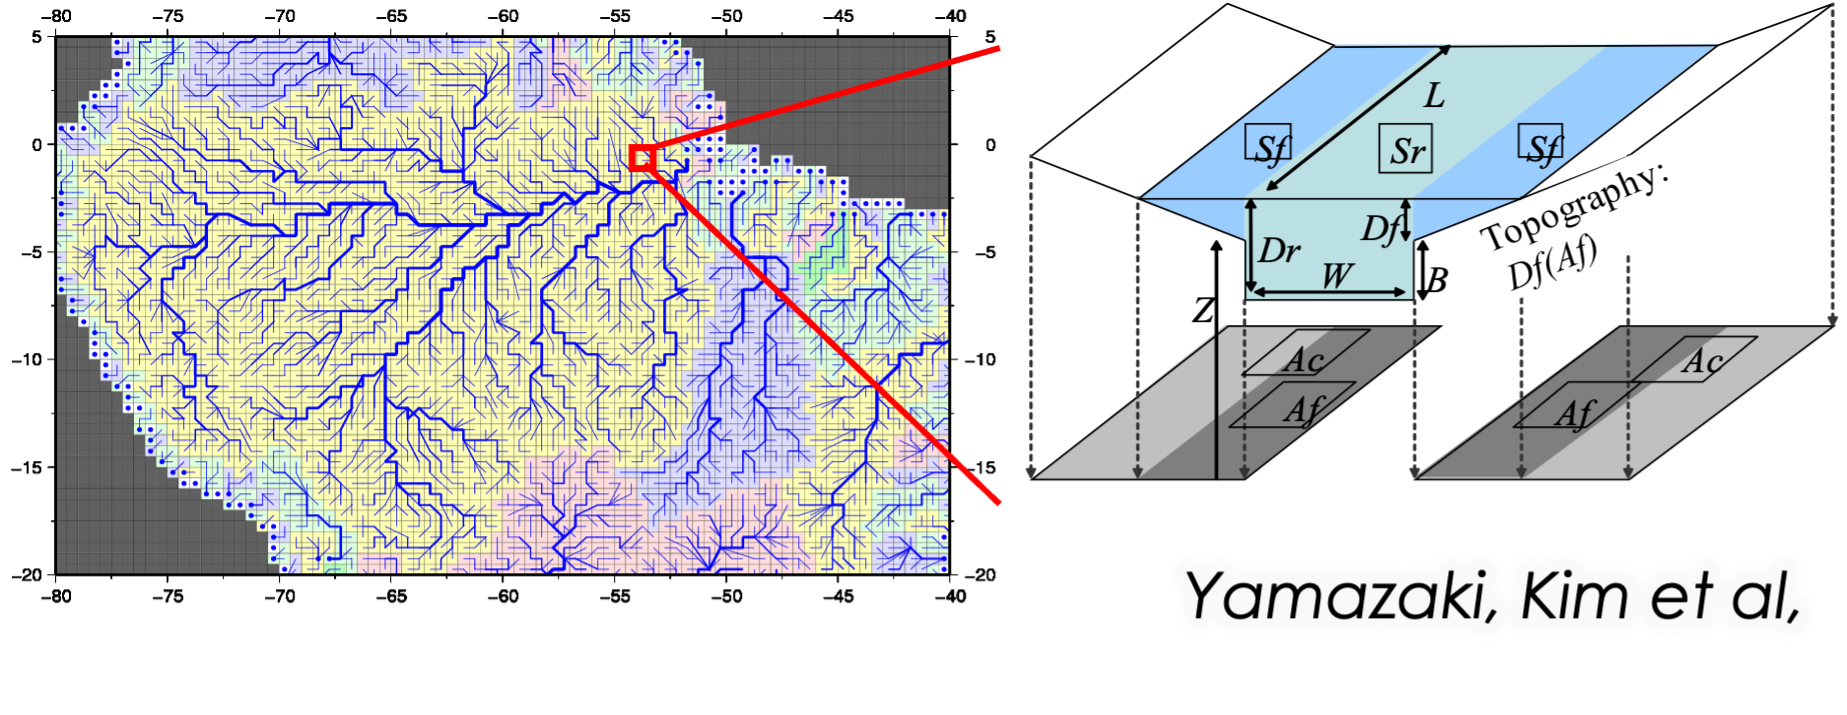
\includegraphics{Figures/陆地表面的水分循环/CaMa-Flood流域单位示意图.png}
\caption{CaMa-Flood流域单位示意图,摘自\citet{yamazaki2011physically}。 }
\label{fig:CaMa-Flood流域单位示意图}
\end{figure}
}

\section{河道径流流量计算}
CaMa-Flood 分别计算了各流域单元向其下游单元的河流径流量和漫滩流量。
二者的计算均通过忽略如下 St. Venant 动量方程式第二项,得到径流计算所使用的局部惯性方程 \cite{bates2010}:
\begin{equation}
\frac{\partial Q}{\partial t}+\frac{\partial}{\partial x}\left[\frac{Q^{2}}{A}\right]+\frac{g A \partial(h+z)}{\partial x}+\frac{g n^{2} Q^{2}}{R^{4 / 3} A}=0
\end{equation}
式中$Q$为河流流量 ($\rm m^3s^{-1}$),$A$为水流横截面面积 ($\rm m^2$),$h$为水流深度 (m),$z$为河床高程 (m),
$R$为水力半径 (m),$g$为重力加速度 ($\rm m s^{-2}$),$n$为曼宁摩擦系数($\rm m^{-1/3} s^{-1}$)。
$x$和$t$分别为流动距离和时间。第一项、第二项、第三项和第四项分别表示局部加速度、平流、水面坡度和摩擦坡度。CaMa-Flood模型采用局部惯性方程的显式形式: 

\begin{equation}
Q^{t+\Delta t}=\frac{Q^{t}+\Delta t g A i S}{1+\frac{\Delta t g n^{2}\left|Q^{t \mid}\right|}{R^{4 / 3} A}}
\end{equation}
其中$S$是水面坡度,$Q^t$为当前时刻的流量, $Q^{t+\Delta t}$是单位时间间隔 $\Delta t$ 之后的流量。水力半径 $R$ 近似为水流深度。曼宁系数默认设置为$n=0.03$。
在局部惯性方程计算中可能出现的负向河流量,代表了下游流域单元向当前流域单元的反向水流(回水)。同时为防止当前网格的总的流出量超过蓄水量,
CaMa-Flood 引入限流器的概念:当总出水量大于网格的总库存量时,CaMa-Flood 使用修正系数对径流流量进行修正。


\section{河道径流流量计算}
漫滩流量计算与河道径流流量计算方法相同。
其区别在于漫滩流量包括所使用的水流面积$A$的计算方法是漫滩蓄水量除以河道长度;
水流深度$h$为漫滩深度;漫滩流量的曼宁系数被设置为$n=0.10$。

\section{蓄水量变化计算}
{
\begin{figure}[]
\centering
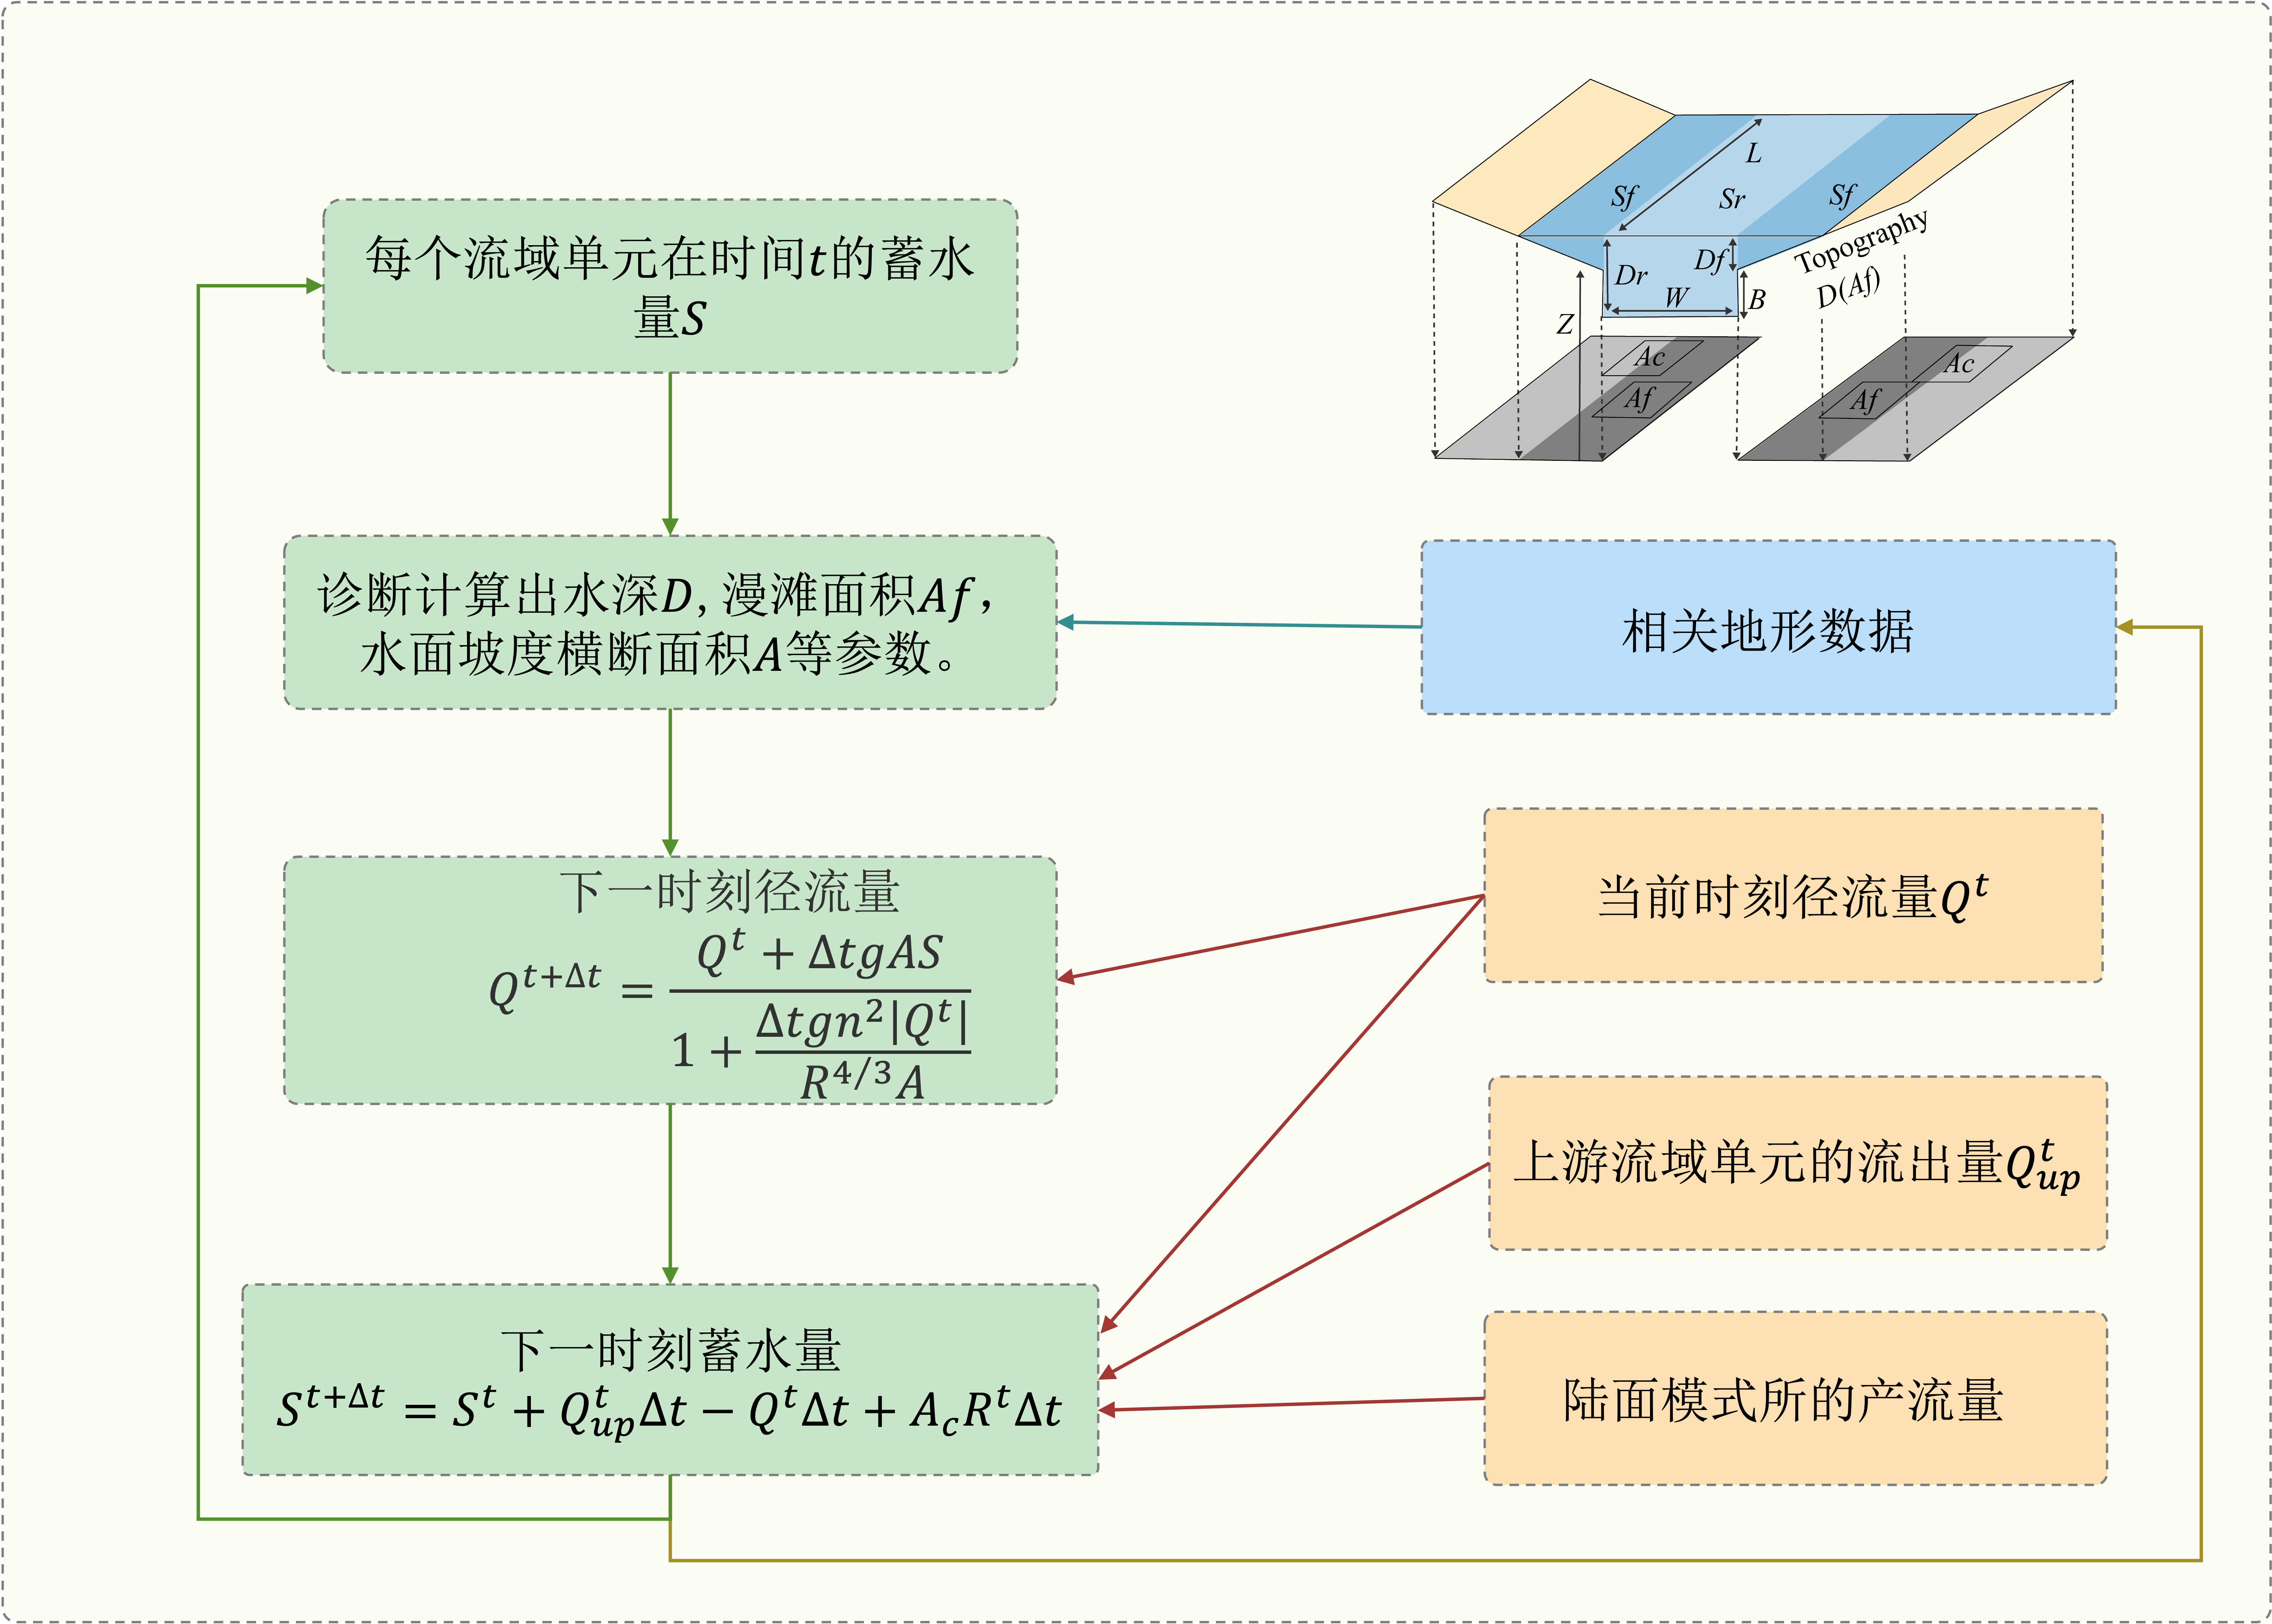
\includegraphics{Figures/陆地表面的水分循环/蓄水量变化计算流程图.png}
\caption{蓄水量变化计算流程图。 }
\label{fig:蓄水量变化计算流程图}
\end{figure}
}
蓄水量随时间的变化的计算流程如图~\ref{fig:蓄水量变化计算流程图}所示,指定流域单元的蓄水量变化的计算基于质量平衡方程:
\begin{equation}
S_{i}^{t+\Delta t}=S_{i}^{t}+\sum_{k}^{Upstream} Q_{k}^{t} \Delta t-Q_{i}^{t} \Delta t+A c_{i} R_{i}^{t} \Delta t
\end{equation}
式中$S_{i}^{t}$和$S_{i}^{t+\Delta t}$分别代表单元$i$在时间$t$到时间$t+\Delta t$蓄水量的变化,$Q_i^t$代表在时间$t$该单元河流径流出流量 (河道内+漫滩),
$Q_k^t$代表在时间 $t$ 该单元从上游网格接收的河流径流流入流量 (河道内+漫滩),$Ac_i$ 是单元$i$的面积,$R_i^t$ 代表流域单元 $i$ 的产流量。

\section{河网地图}
CaMa-Flood 模拟所需的相关次网格地形参数是由 90m 超高精细分辨率的全球流动方向地图 (MERIT-Hydro)\citep{yamazaki2019merit},
水文调整高程 DEM \citep{yamazaki2017high,yamazaki2012analysis},以及河宽数据\citep{yamazaki2014development}; 
使用 \citet{yamazaki2009deriving} 开发的升尺度模式 Flexible Location of Waterways (FLOW) 计算得出。
相关数据以纯``二进制''格式 ($nx*ny$)存储于 \texttt{map/} 目录下。默认的数据存储顺序是从180 \textdegree W到180 \textdegree E,
从 90 \textdegree N 到 90 \textdegree S;数据的字节顺序是 ``little endian''。
具体而言,除了需要陆面模式计算得出的产流量 (runoff) 之外,CaMa-Flood还需要包括流域面积 ($A_s$),河道长度 ($L$),河道宽度 ($W$) 及深度 ($B$),
漫滩 (洪水淹没) 面积,以及用于计算平均漫滩水深的漫滩高程剖面等相关的次网格地形数据。除了河流的宽度和深度以外,
所有的地形相关参数均可由 MERIT-hydro 水文地形数据中获取。以下以全球 0.25\textdegree 的河网为例进行详细介绍。

{
\begin{figure}[]
\centering
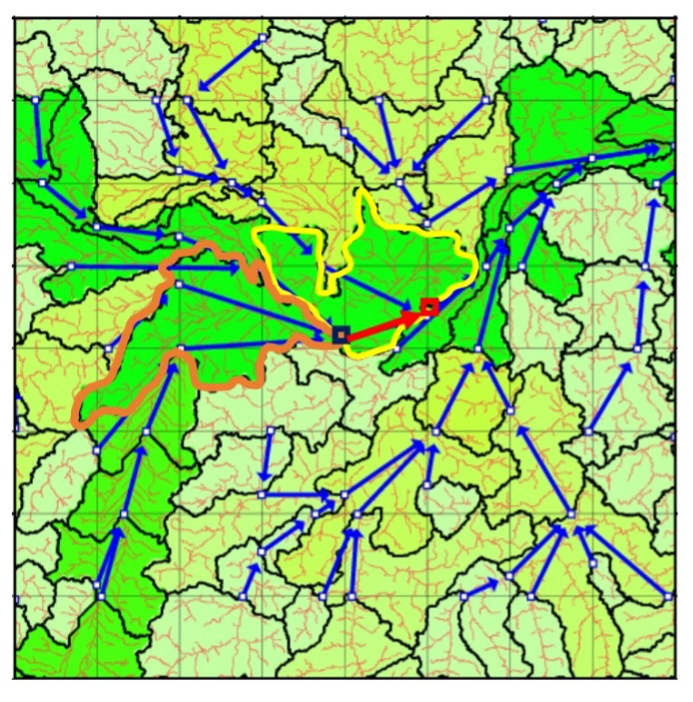
\includegraphics{Figures/陆地表面的水分循环/流域单元分布图.png}
\caption{流域单元分布图。每个流域单元的出口用白色四边形标记。蓝色线条连接不同流域单元,箭头指向下游流域单元。
橙色和黄色边界代表了不同的流域单元。图片摘自\citet{yamazaki2013improving}。 }
\label{fig:流域单元分布图}
\end{figure}
}


在目录\texttt{glb\_15min}下包含了全球 0.25\textdegree 分辨率的网格-矢量-混合 (grid-vector-hybrid) 河网图,
该河网地图是由 90m MERIT Hydro 数据使用 FLOW 模式升尺度而来 (图~\ref{fig:流域单元分布图});
具体文件内容如表~\ref{tab:河网图及地形参数文件列表}和表~\ref{tab:河网图及地形参数文件列表2} 所示。
河网地图的维度信息,包括东西方向网格数目$nx$,南北方向网格数目$ny$,泛滥平原层数 ($nfpl$),
网格大小 ($gsize$)和区域边界 (西、东、南、北),记录在 \texttt{params.txt} 之中。\texttt{nextxy.bin} 文件包含了2个参数 ($nextx$和$nexty$),
分别记录了每个网格的下游单元的相对位置,
其中与海洋接口的河口标记为 -9,内陆河流终点标记为 -10,海洋 (未定义) 标记为 -9999。

% Please add the following required packages to your document preamble:
% \usepackage{booktabs}
\begin{table}[]
\centering
\caption{河网图及地形参数文件列表}
\label{tab:河网图及地形参数文件列表}
    \begin{tabular}[h]{p{3.5cm}p{1.5cm}p{1.5cm}p{5cm}p{1cm}p{1cm}}  %{@{}cccccc@{}}
    \toprule
    File              & Variable & Symbol                        & Description                                  & Unit    & Format  \\ \midrule
    \texttt{params.txt}        & -        & -                             & Map parameters                     & -         & text    \\
    \texttt{nextxy.bin}        & \texttt{nextx}    & $jx$                         & Downstream X (rec=1)         & -         & integer \\
                                       & \texttt{nexty}    & $jy$                         & Downstream Y (rec=2)            & -        & integer \\
    \texttt{downxy.bin}      & \texttt{downx}   & $dx$                        & Relative DownstreamX (rec=1)   & -   & integer \\
                                       & \texttt{downy}   & $dy$                      & Relative Downstream Y (rec=2)   & -    & integer \\
    \texttt{ctmare.bin}       & \texttt{ctmare}   & $Ac$                     & Unit-catchment Area                     & $\rm m^2$   & real    \\
    \texttt{elevtn.bin}        & \texttt{elevtn}    & $Z$                        & Base Elevation                         & m       & real    \\
    \texttt{rivlen.bin}         & \texttt{rivlen}    & $L$                         & Channel Length                        & m       & real    \\
    \texttt{rivhgt.bin}         & \texttt{rivhgt}   & $B$                         & Channel Depth                          & m       & real    \\
    \texttt{rivwth.bin}        & \texttt{rivwth}   & $W$                        & Channel Width                           & m       & real    \\
    \texttt{rivwth\_gwdlr.bin} & \texttt{rivwth}   & $W$                    & Combined Width (recommended)    & m       & real    \\
    \texttt{nxtdst.bin}        & \texttt{nxtdst}   & $X$                             & Downstream Distance                          & m       & real    \\
    \texttt{fldhgt.bin}        & \texttt{fldhgt}   & $D_f$                            & Floodplain Elevation profile (rec=1$\sim$10) & m       & real    \\
    \texttt{rivman.bin}        & \texttt{rivman}   & -                             & Manning’s Roughness                          & -       & real    \\
    \texttt{bifori.txt}        & -        & -                             & Bifurcation Channel Original Data            & -       & text    \\
    \texttt{bifprm.txt}        & -        & -                             & Bifurcation channel parameters               & -       & text    \\ \bottomrule
    \end{tabular}
\end{table}


    % Please add the following required packages to your document preamble:
% \usepackage{booktabs}
\begin{table}[]
\centering
\caption{河网图及地形参数文件列表续}
\label{tab:河网图及地形参数文件列表2}
    \begin{tabular}[h]{p{3.5cm}p{1.5cm}p{1.5cm}p{5cm}p{1cm}p{1cm}} %{@{}cccccc@{}}
    \toprule
    File             & Variable & Symbol                             & Description                                          & Unit     & Format  \\ \midrule
    \texttt{grdare.bin}       & \texttt{grdare}   & -                                  & Rectangular grid area (optional)                     & $\rm m^2$       & real    \\
    \texttt{nxtdst\_grid.bin} &          &                                    &                                                      &          &         \\
    \texttt{rivlen\_grid.bin} & \texttt{nxtdst}   & $X$                                  & Downstream Distance (grid center)                    & m        & real    \\
                                        & \texttt{rivlen}    & $L$                            & Channel Length (grid center)       &    m                             & real        \\
    \texttt{inpmat.bin}       & \texttt{inpx}     & -                                  & Corresponding input grid X (rec=1) & -        & integer \\
                                       & \texttt{inpy}     & -                               & Corresponding input grid Y (rec=2)    & -        & integer  \\
    \texttt{ctmare.bin}       & \texttt{inpa}     & $A_{ij}$                            & Area of input grid XY (rec=3)              & $\rm m^2$     & real    \\
    \texttt{diminfo.txt}      & -        & -                                  & Dimension infomation                         & text     &         \\
    \texttt{lsmask.bin}       & -        & -                                  & Land ID of corresponding hi resolution area Basin ID & -        & integer \\
    \texttt{basin.bin}        & -        & -                                  & Basin ID                                             & -        & integer \\
    \texttt{bsncol.bin}       & -        & -                                  & Basin Color Pattern for Visualization                & -        & integer \\
    \texttt{lonlat.bin}       & \texttt{lon}      & -                                  & Longitude, catchment outlet (rec=1)     & \textdegree      & real    \\
                                     & \texttt{lat}       & -                                 & Latitude, catchment outlet (rec=2)        & \textdegree       & real    \\
    \texttt{uparea.bin}       & \texttt{uparea}   & -                           & Upstream Drainage Area                       & $\rm m^2$        & real    \\ \bottomrule
    \end{tabular}
\end{table}


假设任意网格的洪水事件是从高程低的区域到高程高的区域发生淹没,
任意流域单元(图~\ref{fig:基于流域单元的漫滩高程剖面函数}) 的漫滩面积可以由漫滩水深$D_f$ (m) 
以及累积分布函数 (CDF) 的经验函数生成 (图~\ref{tab:河网图及地形参数文件列表2})。
每个网格的CDF函数的第10百分位数的10个值 (图~\ref{tab:河网图及地形参数文件列表2},红色圆点)分别存储在 \texttt{fldhgt.bin} 的十个参数之中
 (见表~\ref{tab:河网图及地形参数文件列表}和表~\ref{tab:河网图及地形参数文件列表2}),文件格式与上述的 \texttt{nextxy.bin} 相同。
例如,\texttt{fldhgt.bin} 的第三个参数表示流域单元 30\% 的面积被淹没时的该流域单元的平均洪水深度 (m)。

{
\begin{figure}[]
\centering
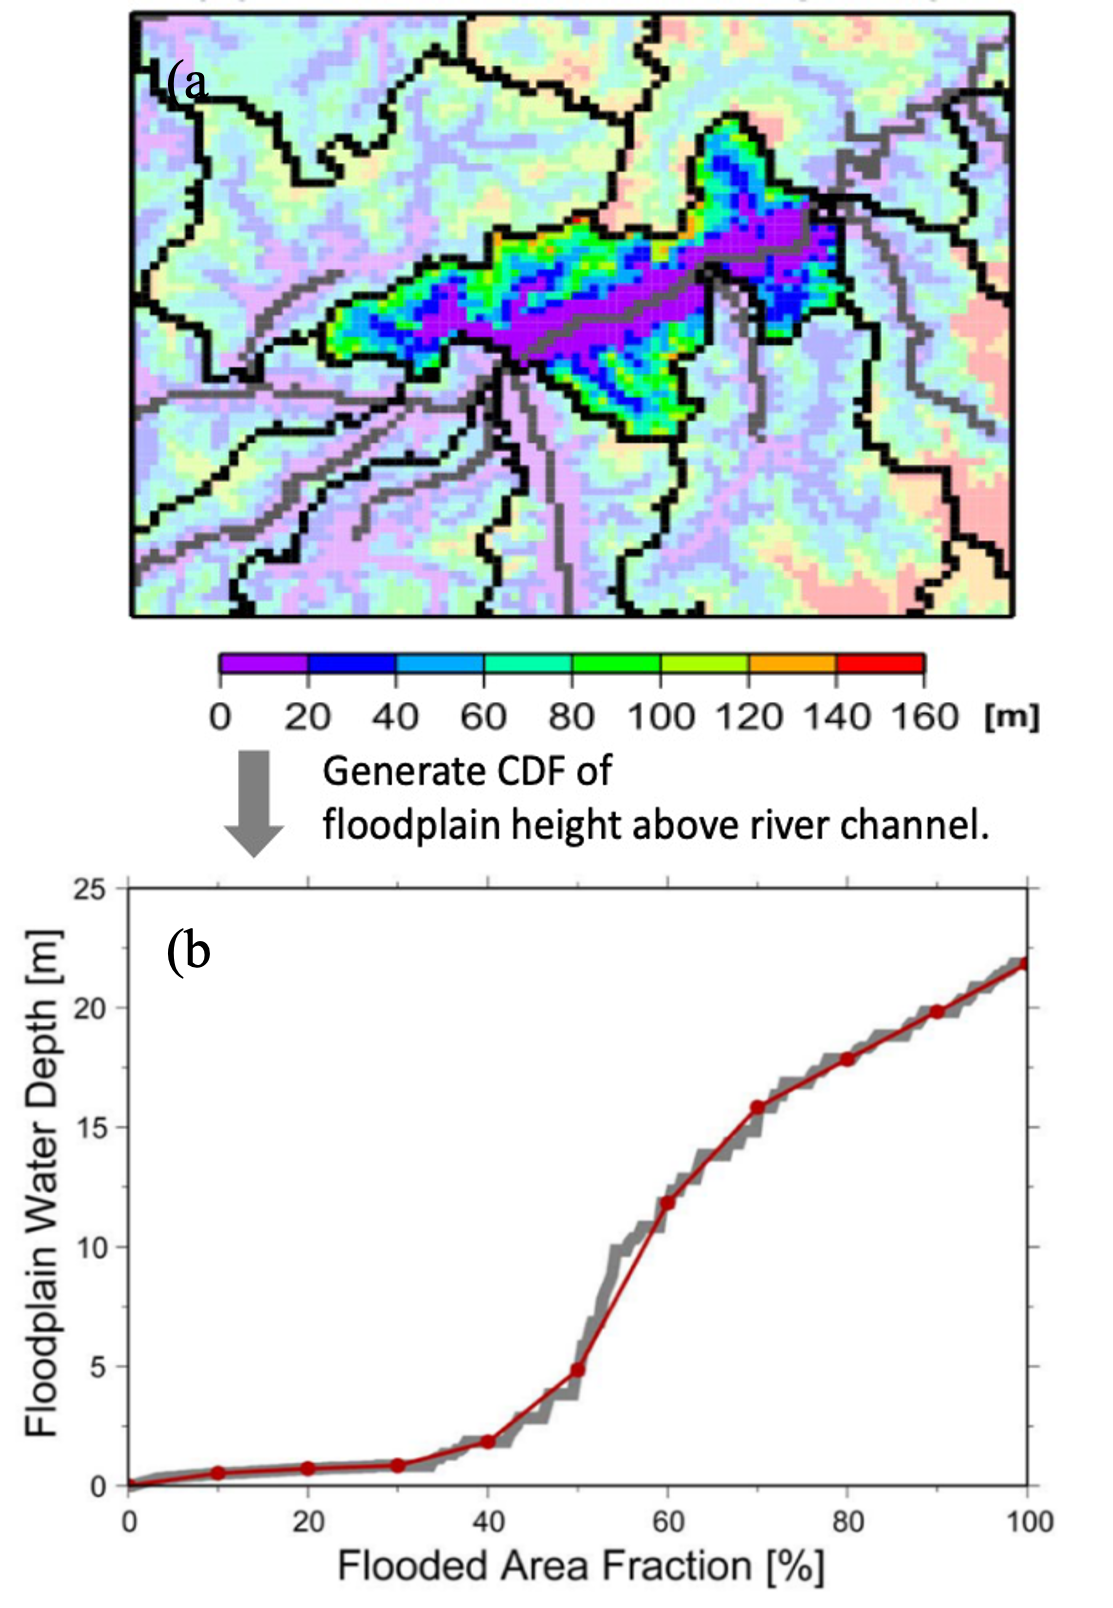
\includegraphics{Figures/陆地表面的水分循环/基于流域单元的漫滩高程剖面函数.png}
\caption{基于流域单元的漫滩高程剖面函数。图片摘自\citet{yamazaki2013improving}。  }
\label{fig:基于流域单元的漫滩高程剖面函数}
\end{figure}
}


河道断面参数(河道长度$W$ (m)和河道深度 $B$ (m))是水动力模拟的主要参数之一。在CaMa-Flood中的该参数是流域产流量的气候态的经验函数,由以下公式推导得出:
\begin{equation}
W=\max \left(W_{min}, c_{w} * Q_{ave}{}^{p_{w}}+W_{0}\right)
\end{equation}
\begin{equation}
B=\max \left(B_{min}, c_{H} * Q_{ave}{}^{p_{H}}+B_{0}\right)
\end{equation}
其中$Q_{ave}$是由陆面模式计算得出的产流量 (total runoff) ($\rm m^3\,s^{-1}$)。
河道宽度计算所使用的经验系数 $c_w$,$p_w$,$W_0$,$W_{min}$ 分别设置为 2.5,0.6,0.0 以及5.0;
河道深度计算所使用的经验系数 $c_H$,$p_H$,$B_0$ 和 $B_{min}$ 分别设置为 0.1,0.5,0.0 以及1.0。
值得注意的是这些经验系数存在着极大的不确定性,在使用之时需要对其进行对应的率定和调参。
除此之外,基于卫星观测的河道宽度数据 (\texttt{width.bin},如图~\ref{fig:基于卫星数据生成的河道宽度示意图}) 也可由MERIT-hydro水文地形数据中获取。
CaMa-Flood推荐使用通过 \texttt{set\_gwdlr.F90} 子程序生成组合宽度参数 (经验公式和卫星数据的组合) 数据。
相关地图的制备详见 \citet{yamazaki2014regional, yamazaki2014development}。
{
\begin{figure}[]
\centering
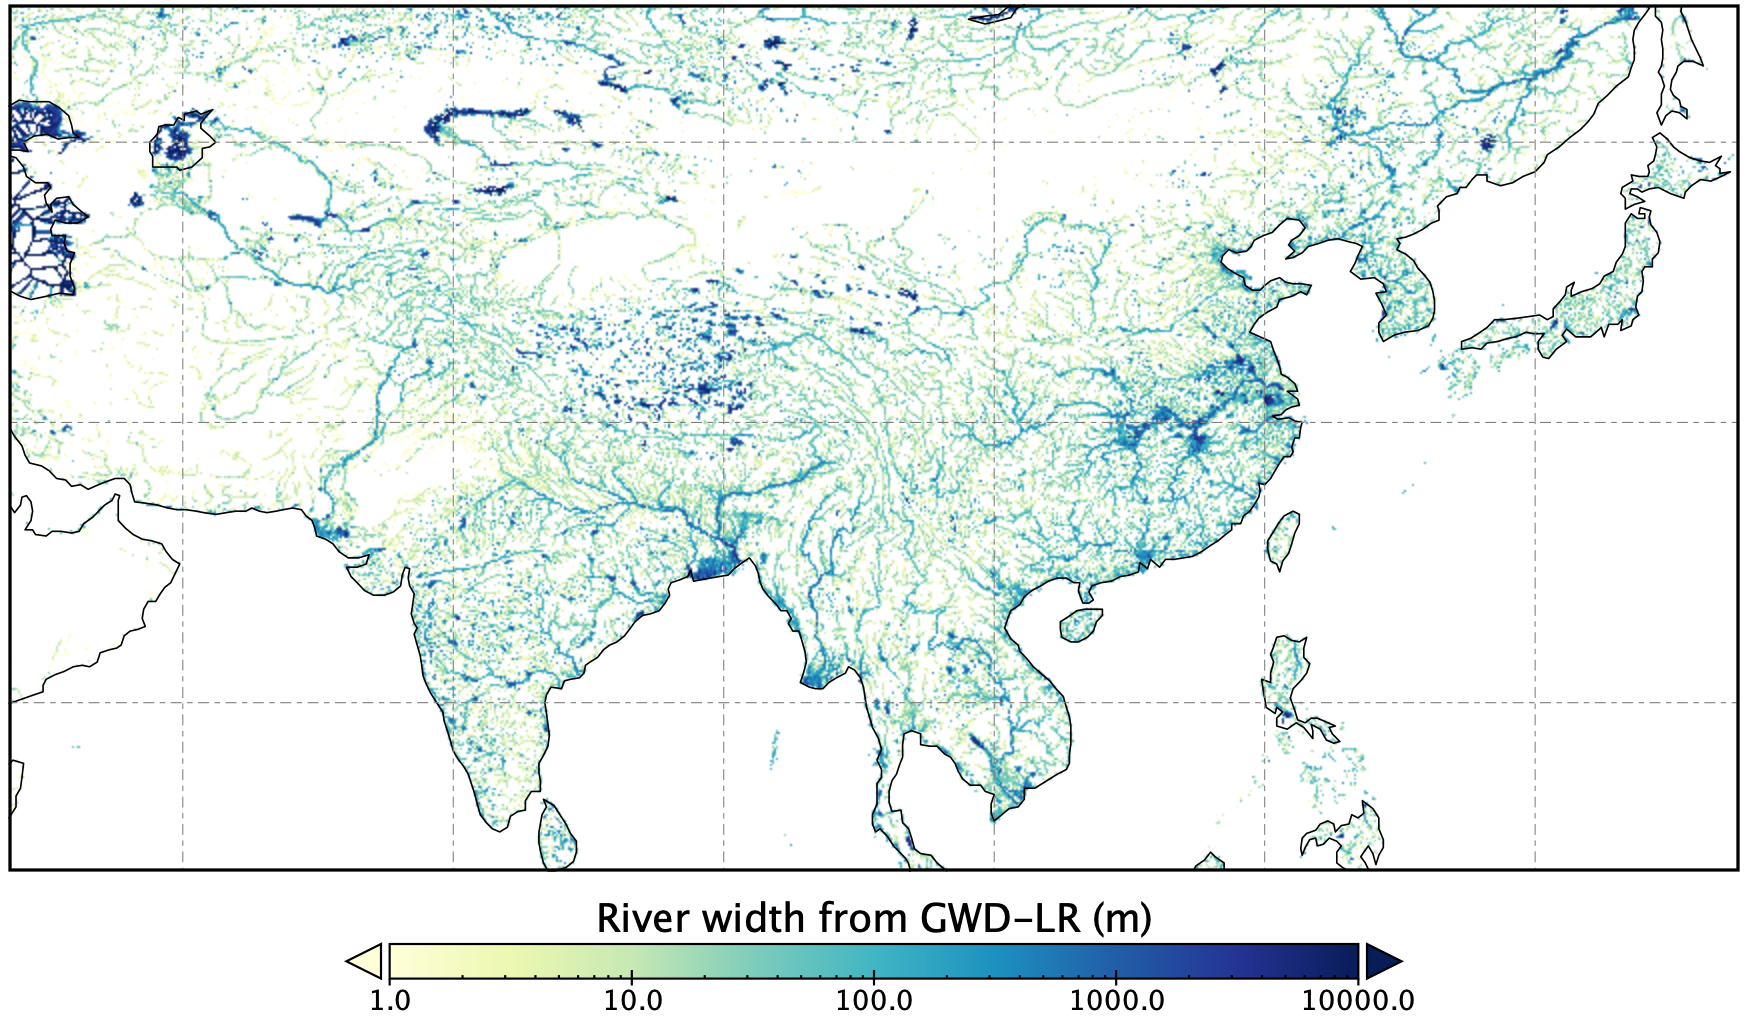
\includegraphics{Figures/陆地表面的水分循环/基于卫星数据生成的河道宽度示意图.png}
\caption{基于卫星数据生成的河道宽度示意图。图片摘自\citet{yamazaki2011physically}。}
\label{fig:基于卫星数据生成的河道宽度示意图}
\end{figure}
}

如图~\ref{fig:CaMa-Flood流域单位示意图} 所示,由于 CaMa-Flood 是基于流域单元进行计算的,而陆面模式是基于规则的经纬度网格,
流域单元在当前陆面模式分辨率 (经纬度网格) 投影下呈现不规则的形状。
因此在流域边缘有可能出现一个网格分属于不同流域,以及多个经纬度网格单元同属于一个流域单元的情况。
这就需要强制插值分割这些陆面模式经纬度网格生成的产流量到不同的流域。
指定流域单元$i$从陆面模式网格获得的水量由如下公式进行计算:
\begin{equation}
F_{i}=\sum_{N} A_{i, j} R_{j}
\end{equation}
其中$F_i$为进入流域单元$i$在单位时间 [$\rm m^3\,s^{-1}$]的输入水量,$A_{i, j}$ 是陆面模式的经纬度网格单元$j$在属于指定流域单元的面积大小,
 $N$是指属于指定流域单元陆面模式的经纬度网格的数量。该映射信息被存储在 \texttt{test\_***.bin} (\texttt{***} 是网格分辨率
 ,例如 \texttt{test\_1deg.bin})。同时,还需准备一个文本文件 (比如说 \texttt{diminfo\_test-1deg.txt}) 用来指定模拟的维度
  (比如说区域,分辨率,流域单元数量,输入经纬度网格数量,输入的映射文件名 \texttt{test\_***.bin})。

在 \texttt{map} 目录中,CaMa-Flood 还准备了一些用于生成映射矩阵和漫滩高程剖面曲线所需的高分辨率数据 (如 \texttt{3sec},\texttt{1min},\texttt{15min},
\texttt{3min} 等目录之下)。
高分辨率数据被划分为\texttt{\$(TILE).\$(VAR).bin},每个TILE的区域记录在 \texttt{location.txt} 文件之中;
具体提供的参数 \texttt{\$(VAR)} 如表~\ref{tab:河网图及地形参数文件列表2} 所示。其中 \texttt{\$(TILE).flwdir.bin} 和
\texttt{\$(TILE).downxy.bin} 分别以基于 D8 格式和 downstreamXY 格式描述了河流流向;\texttt{\$(TILE).catmzy.bin} 表示流域单元内的网格 (ix, iy) 
在高分辨率经纬度网格 (iXX, iYY)上的映射;\texttt{\$(TILE).catmzz.bin} 表示每个网格对应的漫滩层;\texttt{\$(TILE).flddif.bin} 表示每个网格堤坝平均高度 [m],
用于对粗分辨率的漫滩水深进行降尺度;\texttt{\$(TILE).visual.bin} 用于高分辨率流域边界可视化,其中数值上体现为海洋 = 0, 
陆地 (未调整) = 1, 陆地 (调整并在 CaMa 中使用) = 2, 通常网格 = 3,流域边界 = 5, 河道 = 10, 内陆流域出口 = 20, 与海洋连接的河口 = 25。
具体文件列表见表~\ref{tab:河网各数据文件}。

% Please add the following required packages to your document preamble:
% \usepackage{booktabs}
\begin{table}[]
    \centering
    \caption{河网各数据文件}
    \label{tab:河网各数据文件}
    \begin{tabular}[h]{p{4cm}p{1.5cm}p{1.5cm}p{4cm}p{1cm}p{2cm}} %{@{}cccccc@{}} %
    \toprule
    File                & Variable    & Symbol                        & Description                   & Unit      & Format \\ \midrule
    \texttt{location.txt}        & -        & -                             & Hi-res domain info            & -         & text   \\
    \texttt{\$(TILE).catmxy.bin} & \texttt{catmx}    & $iXX$         & catchment (iXX,jYY) rec=1     & - & int*2byte       \\
                                               & \texttt{catmy}    & $jYY$      & catchment (iXX,jYY) rec=2     & - & int*2byte      \\
    \texttt{\$(TILE).catmzz.bin} & \texttt{catmz}    & -                 & floodplain layer              & -  & int*1byte \\
    \texttt{\$(TILE).flwdir.bin} & \texttt{dir}      & -                        & flow direction (D8)         & -   & int*1byte  \\
    \texttt{\$(TILE).downxy.bin} & \texttt{downx}    & $dx$          & relative downstream x (rec=1) & - & int*2byte   \\
                                                & \texttt{downy}    & $dy$       & relative downstream y (rec=2) & - & int*2byte   \\
    \texttt{\$(TILE).elevtn.bin}    & -        & -                             & elevation                     & m                             & real    \\
    \texttt{\$(TILE).flddif.bin}      & -        & -                             & height above river channel    & m                             & real   \\
    \texttt{\$(TILE).rivwth.bin} & -        & -                                & river channel width           & m                             & real   \\
    \texttt{\$(TILE).grdare.bin} & -        & -                               & pixel area                    & $\rm m^2$                            & real   \\
    \texttt{\$(TILE).uparea.bin} & -       & -                               & upstream drainage area        & $\rm m^2$       & real   \\
    \texttt{\$(TILE).visual.bin}  & -        & -                               & Catchment visualization        & -                                                        & int*1byte       \\ \bottomrule
    \end{tabular}
\end{table}
